\documentclass[svgnames,tikz]{standalone}

\usepackage{cmbright,libertine,slashed,physics2}
\usephysicsmodule{ab}
\newcommand \iu {{i\mkern1mu}}

\usetikzlibrary{tikzmark}
\tikzset
  {
    every node/.style =
      { align = center, DarkSlateGray!60, font = \footnotesize },
    every path/.style = { DarkSlateGray!60, line cap = round }
  }

\begin{document}
  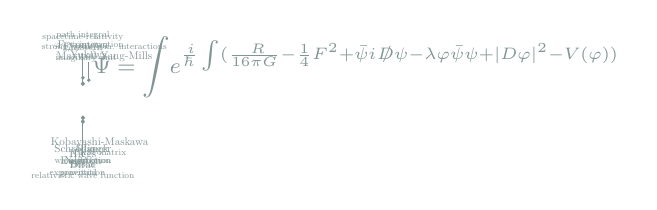
\begin{tikzpicture}
    \node [ above right ] at (0,0)
      { $ \displaystyle
        \tikzmarknode a \Psi = \tikzmarknode b \int
        \tikzmarknode c e^
          {
            \frac { \tikzmarknode d \iu } { \tikzmarknode e \hbar }
            \int \ab(
                \frac { \tikzmarknode f R } { 16\pi \tikzmarknode g G }
              - \frac14 \tikzmarknode h F ^2
              + \bar\psi \iu \tikzmarknode i { \slashed D } \psi
              - \tikzmarknode j \lambda
                \tikzmarknode k { \varphi \bar\psi } \psi
              + |D \tikzmarknode l \varphi|^2 - V(\varphi)
            )
          }
      $};
    \draw ([yshift = -.75ex] a.south) coordinate (A) --++ (0,-.3)
     node [ scale = .4, below ]
      { \normalsize Schr\"odinger\\ wave function };
    \draw ([yshift = .75ex] b.north) coordinate (B) --++ (0,.3)
     node [ scale = .4, above ]
      { path integral\\\normalsize Feynmann };
    \draw ([yshift = -.75ex] c.south) coordinate (C) --++ (0,-.45)
     node [ scale = .4, below, xshift = -2ex]
      { \normalsize  Euler\\ exponential };
    \draw ([yshift = .75ex] d.north) coordinate (D) --++ (0,.225)
     node [ scale = .4, above, xshift = 1ex] { imaginary unit };
    \draw ([yshift = -.75ex] e.south) coordinate (E) --++ (0,-.3)
     node [ scale = .4, below, xshift = 2ex]
      { \normalsize Planck\\ quantum };
    \draw ([yshift = .75ex] f.north) coordinate (F) --++ (0,.375)
     node [ scale = .4, above ]
      { spacetime-relativity\\\normalsize Einstein };
    \draw ([yshift = -.75ex]g.south) coordinate (G) --++ (0,-.45)
     node [ scale = .4, below ] { \normalsize Newton\\ gravitation };
    \draw ([yshift = .75ex] h.north) coordinate (H) --++ (0,.225)
     node [ scale = .4, above, xshift = 4.5ex ]
      { strong/weak/e.m. interactions\\\normalsize Maxwell Yang-Mills};
    \draw ([yshift = -.75ex] i.south) coordinate (I) --++ (0,-.45)
     node [ scale = .4, below ]
      { \normalsize Dirac\\ relativistic wave function };
    \draw ([yshift = -.75ex] j.south) coordinate (J) --++ (0,-.2)
     node [ scale = .4, below, xshift = 3.5ex]
      { \normalsize Kobayashi-Maskawa\\ CKM matrix };
    \draw ([yshift = .75ex, xshift = .5ex] k.north) coordinate (K) --++ (0,.225)
     node [ scale = .4, above ]
      { $\varphi$ - $\psi$ interaction\\\normalsize Yukawa };
    \draw ([yshift = -.75ex] l.south) coordinate (L) --++ (0,-.3)
     node [ scale = .4, below ] { \normalsize Higgs\\ Boson};
    \foreach \x in {A,B,...,L}
      \fill [ DarkSlateGray!60 ] (\x) circle (.025);
  \end{tikzpicture}
\end{document}
